\documentclass[letterpaper,twocolumn,superscriptaddress,showkeys]{revtex4-1}
\usepackage[utf8]{inputenc}
\usepackage{color,dcolumn,graphicx,hyperref}
\hypersetup
{
    colorlinks = true, linkcolor = blue, citecolor = blue, urlcolor = blue,
}

\begin{document}

\title{Developing a preprint culture in biology}

\author{Philippe Desjardins-Proulx}
\email[E-mail: ]{philippe.d.proulx@gmail.com}
\affiliation{Theoretical Ecosystem Ecology laboratory, Universit\'e du Qu\'ebec \`a Rimouski, Canada.}
\affiliation{Quebec Center for Biodiversity Science, McGill University, Canada.}
\affiliation{D\'epartement des sciences biologiques, Universit\'e du Qu\'ebec \`a Montr\'eal, Canada.}

\author{Ethan P. White}
\affiliation{Departement of Bology, Utah State University, United-States of America.}

\author{Joel J. Adamson}
\affiliation{Ecology, Evolution and Organismic Biology, University of North
Carolina at Chapel Hill, United-States of America}

\author{Timoth\'ee Poisot}
\affiliation{Theoretical Ecosystem Ecology laboratory, Universit\'e du Qu\'ebec \`a Rimouski, Canada.}
\affiliation{Quebec Center for Biodiversity Science, McGill University, Canada.}
\affiliation{International Network for Next-Generation Ecology.}

\author{Karthik Ram}
\affiliation{Environmental Science, Policy, and Management. University of California, Berkeley. Berkeley, CA. United-States of America.}

\author{Dominique Gravel}
\affiliation{Theoretical Ecosystem Ecology laboratory, Universit\'e du Qu\'ebec \`a Rimouski, Canada.}
\affiliation{Quebec Center for Biodiversity Science, McGill University, Canada.}

\keywords{Publishing; preprint server; Green Open Access; arXiv.}

% No abstract needed.

\maketitle

\section{Introduction}

Public preprints servers allow authors to make their manuscripts publicly
available before, or in parallel to, submitting them to journals for traditional
peer-review. The idea behind preprint servers is fundamentally simple: to make
the results available to the scientific community as soon as possible rather
than wait until the peer-review process is fully completed. The point of arXiv
and open preprints servers is not to avoid the peer-review process. Almost all
manuscripts on arXiv are submitted to peer-review.  The point is that sharing
ideas as quickly as possible using preprint servers has numerous advantages.
These include rapid dissemination of work in progress to a wider audience, not
only scientists and the general public but also readers in developing countries
where access to subscription journals are often a limiting factor. Furthermore,
preprints provide the opportunity to solicit feedback from a larger pool of
reviewers and can be seen as an integral aspect of a vigorous peer-review
process \cite{hoc12}. Thus, preprint servers increase the number of
opportunities for review and revision prior to publication, resulting in higher
quality submissions which could also alleviate reviewer burden.

The idea gained popularity 20 years ago with the advent of arXiv, an open
preprint server widely used in physics and mathematics \cite{gin11}.  It is also
part of other fields' culture. Paul Krugman noted that, in economics, the
\emph{traditional model of submit, get refereed, publish, and then people will
read your work broke down a long time ago. In fact, it had more or less fallen
apart by the early 80s} \cite{kru12}. In addition to a section in arXiv,
economists have also the RePEc (Research Papers in Economics) initiative, which
aims to create an archive of working papers, manuscripts, and book chapters.
Yet, despite the success of the approach in other fields of inquiry, most
manuscripts in biology are never submitted to any public archive.  In this
article, we will first highlight the advantages of open preprints servers for
both scientists and publishers. We will also debunk a few misconceptions,
discuss the policies of major publishers in biology, and briefly review the most
popular open preprint servers.

\section{The case for open preprints}

The first and most often discussed advantage of arXiv and open preprints is
speed \ref{fig:map}. The time between submission and the official publication of
a manuscript can be measured in months, sometime in years. For all this time,
the research is only known to a select few: colleagues, editors, reviewers.
Thus, the science cannot be used, discussed, or reviewed by the wider scientific
community. It is a problem for both scientists and publishers. Manuscripts that
are unknown cannot be integrated and thus take more time to be cited. It has
been shown that high-energy physics, with its high arXiv submission rate, had
the highest immediacy among physics and mathematics \cite{pra05}.

Furthermore, the review process as a whole is critically over-loaded, because
the number of active scientists increases, because the pressure to publish
increases, and because of an effect dubbed ``the tragedy of the reviewers
commons'' REF.  At the same times, rejection rates are high in most journals
(REF), and when not invited to submit a revision, authors must start the whole
process all over again. It's thus no surprise that different initiatives emerged
over the last few years to decrease the time spent in review. XXX et coll.
(REF) called for the recycling and reuse of peer-reviews: by attaching previous
reviews and detailed replies to a new submission, both the editor and the
referees can gauge the work done on the manuscript, and perhaps evaluate it with
less prejudice. In a similar way, the \emph{Peerage of Science} initiative
allows authors to seek anonymous pre-review by their peers. Some journals now
accept to publish papers which received good evaluations, with \emph{Animal
Biology} having recently accepted first a paper reviewed entirely with the
\emph{Peerage of Science} \cite{abb12}, effectively outsourcing the review
process. A widespread use of preprint servers can achieve the same goal of
reducing the time spent in review. By putting a manuscript for open comments and
criticisms, the authors will receive valuable feedback and can improve the
version which will be submitted. With a rich enough community of scientists
depositing preprints, and commenting on them, the process of an open pre-review
can become widespread and will overall increase the quality of first
submissions.

\begin{figure}[ht!] \centering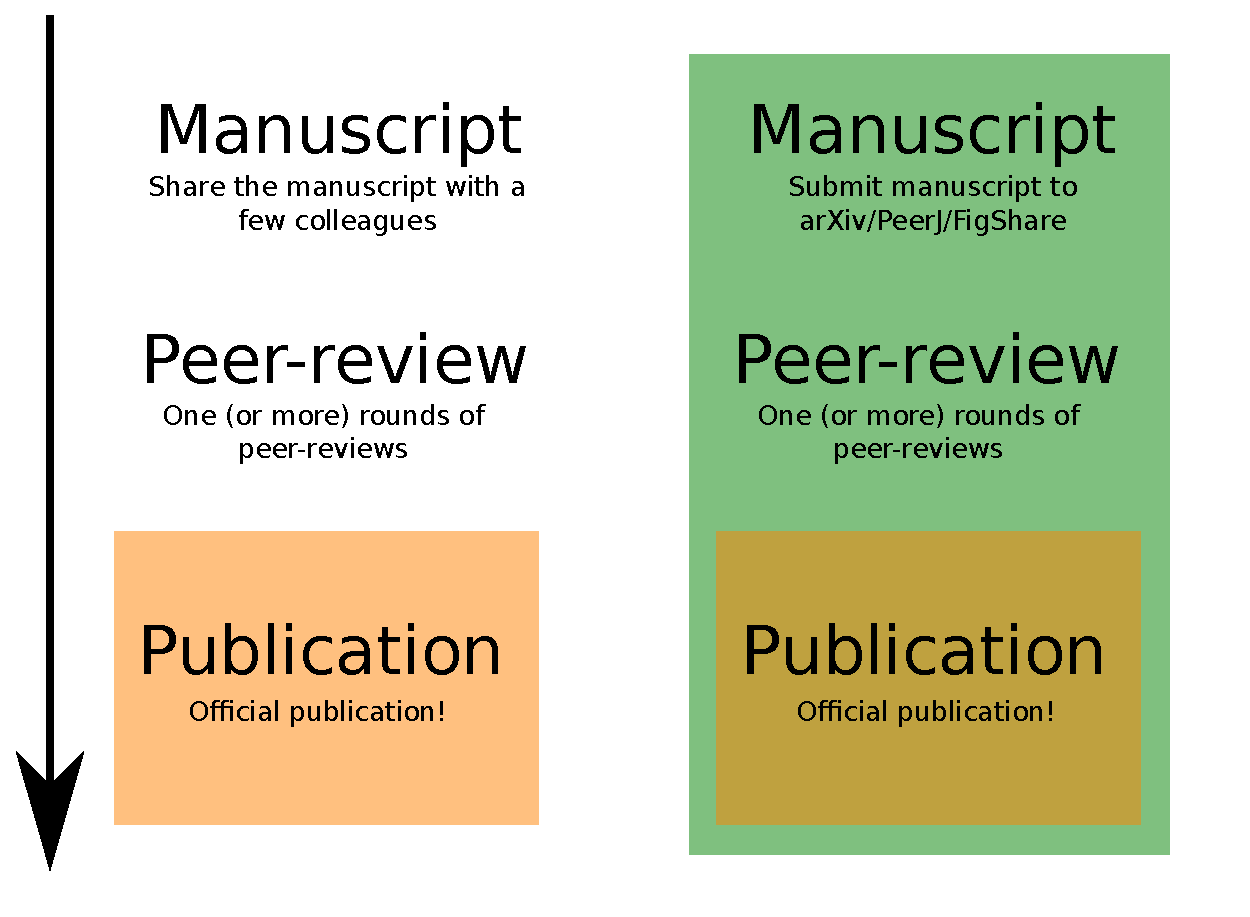
\includegraphics[width=0.50\textwidth]{map.pdf}
\caption { It can take several months, and even a few years, before a submitted
paper is officially published and citable.  The average time to publication
varies greatly between journals and can be as low as 104 days (Evolution for
2011) to 213 (PLOS One in 2010).  Meanwhile, few people are aware of the
research that has been done since, typically, only close colleagues are given
access to the preprints. With public preprint servers, the science is
immediately available and can be openly discussed, analyzed, and integrated into
current research. It benefits both science and publishers. Both want the papers
to be well-known and cited, and public preprints make it possible to integrate
research even before publication, greatly improving immediacy.  }
\label{fig:map} \end{figure}

Public preprint servers offer a much fairer way to establish intellectual
priority by making the work available when done. Some manuscripts will spend
much more time in the review process than others. Surprisingly, there is a
perception in biology that public preprints make it easier to steal ideas, as if
a scientific idea was only complete once published in a peer-reviewed journal.
Mathematicians and physicists have embraced arXiv in part to establish priority
in a fair way and biologists should do so too, or at least not be afraid to
submit to make their research public for fear of been snooped \cite{cal12}.

Prepublication reviews by a small network of colleagues is an important part of
the scientific process, which is attested by the fact that nearly all published
papers acknowledge comments by people not listed as co-authors.  Preprint
servers simply offer a way to extend this network of colleagues to the entire
scientific community. It ensures that science is not constrained by small
networks of scientists exchanging ideas.  Paul Ginsparg created arXiv.org in
part for democratic reasons: he wanted everyone from students in small
universities to Ivy-League professors to have access to the most recent
scientific \emph{ideas}.  Ginsparg's revolutionary idea was simply to use the
power of the internet for preprints, not just for the end product, so the
scientific process can be open as soon as possible.

\section{Preprints in biological sciences}

Submitting to a preprint server is becoming more common in biology, even though
it still involves a minority of papers. The quantitative biology section in
arXiv is experiencing faster growth in submissions than any other field
\cite{cal12}. Also, most scientific journals are preprint-friendly: Nature,
PLOS, BMC, PNAS, Science (mostly) \ref{table:policies}, and all the journals
from Elsevier and Springer. Very recently, the Ecological Society of America and
the Genetics Society of America changed their policies to allow public
preprints. Few scientific publications will not consider a manuscript submitted
to a public preprint server.  Still, a few journals adopt a ``by default''
hostile attitude towards preprints, mostly due to the lack of clear policy of
the publishers, or perhaps because a preprint culture has not developed in
biology and the practice is still considered unusual. As an example,
Wiley-Blackwell, which publishes some leading journals, has no official policy
on the subject \ref{table:policies}.

\begin{table*}
    \centering
    \begin{tabular}{|ll|}
    \hline
    Publisher                                   & Policy \\
    \hline
    Springer                            	& Accept \\
    BMC                                 	& Accept \\
    Elsevier                            	& Accept \\
    Nature Publishing Group             	& Accept \\
    Public Library of Science           	& Accept \\
    Genetics Society of America                 & Accept \\
    Royal Society                       	& Accept \\
    National Academy of Science (USA)           & Accept \\
    Ecological Society of America       	& Accept \\
    Oxford Journals                             & Accept \\
    Science                             	& Ambiguous \\
    Wiley-Blackwell                       	& No general policy \\
    British Ecological Society                  & No answer to our query \\
    \hline
    \end{tabular}
    \caption{Policies for important publishers in biology. Some publishers
tolerate preprints except for a few of their medical journals, e.g.: Journal
of the National Cancer Institute from Oxford and The Lancer from Elsevier.}
    \label{table:policies}
\end{table*}

% Not sure about this paragraph, as much as I love to hate MS Office, I would
% rather keep the thing as a "pro-preprint" paper only and not use it to promote
% LaTeX/R.
% -- PhDP

%There are other barriers to adoption of preprint servers by biologists.  The
%most notable preprint server, arXiv, is designed to work best with \LaTeX, the
%dominant document preparation system among physicists and mathematicians.
%Jackson \cite{jackson2002preprints} argues that \LaTeX introduced an
%open source mindset to its users, who now freely share their research
%findings as well as their software.  Many biologists instead use proprietary
%software to prepare their research findings, and many journals officially prefer
%Microsoft Word documents as submissions.  The recent discipline-wide adoption of
%free software packages such as R and associated document generation systems
%\cite{xie2012}, as well as interest in open access publishing, has coincided
%with recent rise in use of preprint servers by biologists, supporting Jackson's
%claims \cite{xie12}.

\section{Current offerings}

We briefly discuss the main options to submit preprints to open servers:
arXiv.org, Figshare, and the upcoming PeerJ and F1000Research.

\subsection{arXiv}

arXiv (\url{http://arxiv.org/}) is the most widely-used preprint server today,
and its use is almost universal in some branches of mathematics and physics.  It
provides a reliable citation system for all eprints and is especially popular in
high-energy physics. Physicist Paul Ginsparg created arXiv in 1991 for
theoretical high-energy physicists to communicate preprints via email and ftp,
and soon thereafter adopted the newly created world-wide
web\cite{jackson2002preprints}.  arXiv now receives over 7,000 submissions per
month (\url{http://arxiv.org/show_monthly_submissions}) and divides its
submissions into subcategories of physics, mathematics, computer science,
quantitative biology, finance and statistics.  The quantitative biology category
includes subcategories for Populations and Evolution, Quantitative Methods and
other categories that may be of interest to biologists.

Submission to arXiv is fully automated.  Authors can submit \TeX/\LaTeX
documents that are compiled on the server or directly submit in PDF/PS format
(for example, as exported by a word processor).  A moderation system was put in
place in 2004: papers must be categorized by an endorser. At least one
author of a paper must be an endorser that has previously submitted a paper or
has received permission to submit to a particular category.  Many authors in
mathematics and physics submit papers as soon as they are ready for review by
colleagues, although another popular option is submitting simultaneously to a
journal and arXiv.

% To review: 
To submit to arXiv, the authors must either have their work available under an
open license or grant arXiv a non-exclusive and irrevocable license to
distribute the article. In either case, arXiv does not require copyright
transfer and only requires the rights to distribute submitted articles in
perpetuity. Thus, submitting to arXiv does not in itself prevent the authors
from transferring their rights to a publisher, which is why most publishers
tolerate arXiv, even though they ask the authors to transfer their right to them
upon acceptance of the article. 

Most papers posted to arXiv are eventually printed in journals but there are
notable exceptions, such as Perelman's landmark paper leading to the proof of
the Poincar\'{e} conjecture \cite{2002math.....11159P}. Yet, arXiv has never
sought to replace scientific journals and explicitly states that it serves a
different function as ``an openly accessible, moderated repository for scholarly
articles in specific scientific disciplines.'' arXiv is now administered by the
Cornell University Libraries, with funding coming from voluntary pledges by academic
institutions along with matching funds from the Simons Foundation
\cite{arxiv_future}.  One-hundred twenty six of the top two-hundred institutions
in terms of downloads have provided the operating budget for arXiv over the next
five years.  This plan reduces the financial burden on Cornell University and
transfers governance to a collaborative community in accordance with arXiv's key
principles.  arXiv takes numerous measures to ensure that the repository will
remain permanently available and submissions will be readable.

\subsection{Figshare}

Figshare (\href{http://figshare.com/}{http://figshare.com/}) is an open server
that allows scientists to submit any research output: manuscript, figures,
datasets, videos, theses, presentations, and so on. There are no rules to limit
what constitutes a research output and, unlike arXiv, there is no endorser
system. All figshare content has a unique digital object identifier (DOI) like
any journal article, thus offering a permanent and stable link to the content.
A flexible tag system is used to classify each item. All content can be
commented and is licensed under the Creative Commons (CC-BY) license, except
datasets which are published under CC0.

One of the biggest advantage of figshare over arXiv is that is it not limited to
quantitative sciences. arXiv.org has sections on quantitative biology but might
not be appropriate for non-quantitative work. With its flexible approach to
preprints, figshare offer an important alternative to arXiv for empirical
biologists. Furthermore, by allowing all 

\subsection{PeerJ}

% @Ethan

\subsection{F1000Research}

F1000Research is not a public preprint server like the previous three servers.
Whereas arXiv, Figshare, and PeerJ offer an option to submit a manuscript
without having it reviewed, papers submitted to F1000Research will eventually be
reviewed. Thus, F1000Research offers a hybrid model with publicly available
manuscripts at time of submission and standard peer-reviews. Manuscripts are
considered ``accepted'' and will only be indexed after two positive referee
response.

\subsection{Github et al.?}

This manuscript was developed entirely as an open project on github. github is a
hosting service for projects under the git revision control tool. git is a
decentralized revision control system used primarily to develop software. It
allows the users to share code, track changes, and merge versions. For example,
during the development of this manuscript, one author would fork the project
(that is: make a personal copy), modify it, and then the changes were merged
back into the main branch. These techniques are widely used in open source
software development. It goes even farther than submitting preprints by opening
the entire writing process. 

\section{Conclusion}

Responding to the rumour that they refused manuscripts submitted to arXiv,
Nature responded that ``Nature never wishes to stand in the way of communication
between researchers. We seek rather to add value for authors and the community
at large in our peer review, selection and editing'' \cite{nat05}.

Open preprints server offer a great opportunity for open science, especially if
the community embrace the idea of discussing preprints. Initiatives like
Haldane's Sieve (\href{http://haldanessieve.org/}{http://haldanessieve.org/}), a
new blog discussing arXiv papers in population genetics, will help make arXiv
attractive for scientists looking to promote their work. These initiatives are
important to fully exploit the potential of open preprints servers.

Posting preprints online increases the community of available informal peer
reviewers, and uses the internet for its original community-building purposes.
Preprint servers also facilitate communication between disciplines, bridging
cultural as well as geographic divides. The advantages are clear and the costs
are low.

Physicists and other quantitative scientists have recently developed a great
interest in evolutionary theory, quantitative ecological theory and
epidemiological modeling.  Unfortunately this has led to a lot of repeated work
(``reinventing the wheel''; \cite{de2011contribution}) that could be avoided by
better communication across disciplines.  The near-universal adoption of
preprint servers in physics provides this vital communication channel.  We
suggest that biologists reach out to physicists and mathematicians by posting
papers to arXiv: a physicist who does not read \emph{Evolution} certainly checks
arXiv at least weekly.  This benefits both disciplines, as biologists will reach
new readers, and physicists will learn the terminology, tools and ideas common
in existing evolutionary theory.  A recent series of papers on the theory of
natural selection was posted to arXiv simultaneously with its publication in the
\emph{Journal of Evolutionary Biology}
\cite{JEB:JEB2431,JEB:JEB2498,JEB:JEB2378,JEB:JEB2373}.

\section{Funding}

PDP is funded by an Alexander Graham Bell scholarship from the National Sciences
and Engineering Council of Canada.

DG is funded by a Discovery Grand from the National Sciences and Engineering
Council of Canada and by the Canada Research Chair program.

\section{Acknowledgements}

...

\newpage
\bibliography{refs}
\bibliographystyle{plain}

\end{document}

